\documentclass{beamer}

\usetheme{Frankfurt}

\usepackage[utf8x]{inputenc}
\usepackage[ngerman]{babel}
\usepackage{subfigure}
\usepackage{caption}
\usepackage{listings}
\lstdefinelanguage{diff}
{
    morekeywords={+, -},
    sensitive=false,
    morecomment=[l]{//},
    morecomment=[s]{/*}{*/},
    morecomment=[l][\color{darkgreen}]{+},
    morecomment=[l][\color{red}]{-},
    morestring=[b]",
}


% draw
%\usepackage[rgb]{xcolor}
\definecolor{hublue}{rgb}{  0, .21, .42}
\definecolor{darkred}{rgb}{.5, 0, 0}
\definecolor{darkgreen}{cmyk}{0.7, 0, 1, 0.5}
\definecolor{darkblue}{rgb}{0, 0, .5}

\usepackage[lflt]{floatflt}

\setbeamertemplate{footline}{%
  \usebeamerfont{date in head/foot}
%  \insertshortauthor - \inserttitle{}\hfill
%  \usebeamertemplate{navigation symbols}\hfill
  \insertframenumber{}/\inserttotalframenumber}
\setbeamertemplate{sidebar right}{}


\title{Using DisplayLink Devices with OpenWRT}
\institute[{Humboldt-Universität zu Berlin}]{\inst{}Humboldt-Universität zu Berlin}
\author[Magnus Müller \and Kai Warnicke \and Dominik Oepen]{Magnus Müller \and Kai Warnicke \and Dominik Oepen}
\date[16.02.2011]{16. Februar 2011}

\begin{document}
	\begin{frame}
		\titlepage
	\end{frame}

	\begin{frame}
		\frametitle{Overview}
		\tableofcontents
	\end{frame}	

	\section{Displaylink}
	
	\begin{frame}
		\frametitle{Mimo 720f}
		\begin{center}
			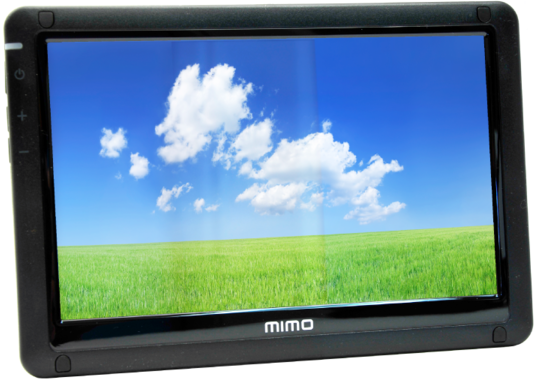
\includegraphics[scale=0.3]{img/mimo720f}
		\end{center}
		
		\begin{itemize}
			\item 7 Zoll Bildschirmdiagonale, Auflösung 800*480
			\item USB-Powered
			\item Touchscreen
		\end{itemize}
	\end{frame}
			
	\begin{frame}
		\frametitle{Displaylink und OpenWRT}
		\begin{itemize}
			\item Backfire: Display funktioniert nach Kernelkonfiguration, aber kein Touch
			\item Benötigt aktuelleren Kernel. 2 Optionen:
				\begin{enumerate}
					\item Neueren Kernel in Backfire einbinden
					\item Developer-branch nutzen
				\end{enumerate}
		\end{itemize}
	\end{frame}

	\section{Touchscreen}
	
	\section{Qt}
	
	\begin{frame}
		\frametitle{Qt}
		\begin{floatingfigure}[l]{1.75cm}
			
\includegraphics[scale=0.3]{img/qt-logo}
		\end{floatingfigure}
		
		Qt is a cross-platform application  and UI framework used by hundreds of thousands of developers worldwide looking to create amazing user experiences  on Windows, Mac, Linux/X11, embedded Linux, Windows CE , Windows Mobile, Symbian  and Maemo devices.
	\end{frame}	
	
	\begin{frame}[containsverbatim]
		\frametitle{Qt patch}
		\begin{lstlisting}[language=diff, basicstyle=\scriptsize]
--- qscreenlinuxfb_qws.cpp.org	2011-02-04 16:11:34.000000000 +0100
+++ qscreenlinuxfb_qws.cpp2011-02-04 16:20:39.741035002 +0100
@@ -337,7 +337,12 @@
         return false;
     }
 
-    d_ptr->driverType = strcmp(finfo.id, "8TRACKFB") ? GenericDriver : EInk8Track;
+    if (!strcmp(finfo.id, "8TRACKFB"))
+        d_ptr->driverType = EInk8Track;
+    else if (!strcmp(finfo.id, "udlfb"))
+        d_ptr->driverType = UDLFB;
+    else
+        d_ptr->driverType = GenericDriver;
 
     if (finfo.type == FB_TYPE_VGA_PLANES) {
         qWarning("VGA16 video mode not supported");
@@ -1252,6 +1257,9 @@
             ioctl(d_ptr->fd, 0x46a2, 1);
         else
             ioctl(d_ptr->fd, 0x46a2, 0);
+    } else if (d_ptr->driverType == UDLFB) {
+        int coords[4] = {r.left(), r.top(), r.right(), r.bottom()};
+        ioctl(d_ptr->fd, 0xAA, &coords);
     }
 }
 
--- qscreenlinuxfb_qws.h.org	2011-02-04 16:12:27.000000000 +0100
+++ qscreenlinuxfb_qws.h	2011-02-04 16:23:11.241035001 +0100
@@ -88,7 +88,7 @@
 
     virtual bool useOffscreen();
 
-    enum DriverTypes { GenericDriver, EInk8Track };
+    enum DriverTypes { GenericDriver, EInk8Track,  UDLFB};
 
     virtual void disconnect();
     virtual void shutdownDevice();	
		\end{lstlisting}
	\end{frame}

\end{document}
